\subsection{Objetivos}

El desarrollo de una PCB se considera una de las partes esenciales de este proyecto y por lo tanto su importancia es máxima.

El objetivo principal que persigue el diseñar y construir una PCB en este proyecto es el de dotar al sistema de un centro de cómputo principal, el cual es utilizado para procesar las ordenes de S1, realizar los cálculos pertinentes y ejecutar las acciones necesarias sobre la estructura del brazo robótico.

Se considera  por lo tanto que la PCB es el centro de computo principal del sistema y por lo tanto se encarga de alojar el microcontrolador DSPIC, así como todos los periféricos necesarios para establecer la comunicación con S1, realizar el control de los actuadores y monitorizar el estado del manipulador.

En los siguientes apartados se detalla el proceso de diseño y construcción llevado a cabo para completar la PCB.

\subsection{Componentes principales}

El diseño de la PCB esta completamente estructurado según varios componentes principales, por lo tanto, en este apartado se describe cuales son, las decisiones que han llevado a incluirlos y sus funcionalidades principales dentro del proyecto.

En general se podría decir que los componentes de la PCB se clasifican en tres categorías principales:
\begin{itemize}
    \item Componentes de alimentación eléctrica.
    \item Microcontrolador y componentes auxiliares para su correcto funcionamiento.
    \item Periféricos destinados a control de actuadores y canales de comunicación.
\end{itemize}

En primer lugar, los componentes de alimentación eléctrica son aquellos que forman el circuito de alimentación del microcontrolador así como de los actuadores. El circuito eléctrico de alimentación de la PCB se ha diseñado para poder alimentar de forma simultánea al microcontrolador y a cada uno de los cuatro servomotores y por lo tanto, está formado por dos etapas:
\begin{itemize}
    \item La PCB recibe una tensión de entrada de 9V y una corriente de entre 1.8A - 2A mediante una clema. Posteriormente esta tensión de alimentación será reducida y adaptada para alimentar a cada una de las etapas de la PCB, es decir, al microcontrolador y servomotores.
    \item En la primera etapa se reduce el voltaje de alimentación principal a 6V y 0.4A aproximadamente para cada uno de los servomotores, utilizando para ello un regulador LM317 para cada servomotor. Esta alimentación se realiza mediante clemas, a las cuales se deben conectar la alimentación de los motores.
    \item En la segunda etapa se reduce el voltaje de alimentación principal a 3.3V y 0.15A aproximadamente con objetivo de alimentar el microcontrolador, utilizando para  ello un regulador LM317. Esta alimentación se realiza mediante pistas únicamente.
\end{itemize}

En segundo lugar, el microcontrolador y sus componentes auxiliares representan el núcleo de la PCB:
\begin{itemize}
    \item El DSPIC se encuentra localizado en el centro de la PCB y de él surgen todas las conexiones necesarias hacia los periféricos.
    \item Los componentes auxiliares del microcontrolador son componentes eléctricos que aseguran el correcto funcionamiento del DSPIC, así como su seguridad. En el caso específico de este microcontrolador, es necesario incluir varios condensadores en sus pines de alimentación.
\end{itemize}

En último lugar se detallan los principales periféricos que serán empleados:
\begin{itemize}
    \item Cristal de cuarzo: mediante este periférico se genera una señal de reloj precisa y de buena calidad, su frecuencia es de 7Mhz y sera recibida por el microcontrolador para ser usada como señal de reloj principal del sistema.
    \item Puerto de programación: mediante este periférico se puede conectar la sonda de programación del microcontrolador y por lo tanto es un elemento esencial.
    \item Puerto TRIS: mediante este periférico se pueden recibir señales digitales y analógicas las cuales son procesadas por el microcontrolador. En este proyecto se utiliza este periférico para monitorizar los finales de carrera de la estructura del brazo robótico.
    \item Puerto PWM: mediante este periférico se pueden generar señales PWM, las cuales son completamente necesarias para controlar los servomotores.
    \item UART: mediante este periférico se establece un canal de comunicación hardware con S1, el cual se usa para recibir ordenes, movimientos y realimentar su resultado de vuelta a S1.
    \item LEDS de estado: mediante este periférico se muestra el estado del sistema usando tres diodos LED.
\end{itemize}

Mediante esta descripción general de la PCB y sus componentes se pretende brindar una idea global de la misma, así como de cual es su papel dentro del proyecto. En los apartados siguientes se describe en términos técnicos los elementos de esta PCB, así como el proceso de diseño y fabricación llevado a cabo.

\subsection{Diseño lógico y diagrama esquemático}

El primer paso llevado a cabo durante el diseño de la PCB ha sido realizar un diseño lógico de alto nivel, en el cual se muestran las conexiones lógicas que existen entre los componentes; se trata por lo tanto del diseño con mayor nivel de abstracción y que tiene como objetivo establecer un diseño de primer nivel, es decir, la primera toma de contacto con el plano de la PCB.

El diseño lógico se lleva a cabo mediante un diagrama esquemático que contiene dos tipos de elementos: huella lógica de cada uno de los componentes y conexiones entre ellos. Este diagrama se ha llevado a cabo utilizando la herramienta Schematic Layout Editor incluida en KiCad.

El diagrama esquemático esta dividido en dos partes principales, las cuales facilitan la compresión del mismo:
\begin{itemize}
    \item Diagrama esquemático del circuito de alimentación.
    \item Diagrama esquemático del microcontrolador y sus periféricos.
\end{itemize}

En primer lugar se procede a describir detalladamente el diagrama esquemático del circuito de alimentación, el cual contiene las dos etapas de alimentación, siendo los principales componentes usados los reguladores de voltaje LM317,L7805CV y AZ1117H.

La clema principal de alimentación recibe 9V y 1.8A aproximadamente. Esta alimentación debe ser provista externamente mediante una fuente de alimentación regulable o similares. 

Conectados directamente a la clema principal se encuentran conectados los reguladores de tensión correspondientes a las dos etapas de alimentación:
\begin{itemize}
    \item La primera etapa de alimentación está formada por cuatro reguladores LM317, los cuales alimentan cada uno de los servomotores. En esta etapa de alimentación se reduce el voltaje de 9V a 5.5V.
    
    \item La segunda etapa de alimentación está formada por un regulador de tensión L7805CV y un AZ1117H. En esta etapa de alimentación se reduce el voltaje de 9V a 5V usando el primer regulador, y de 5V a 3.3V usando el segundo.
\end{itemize}

El funcionamiento del regulador LM317 es bastante común, se trata de un regulador de voltaje ajustable que recibe una tensión continua de entrada de entre 3V - 40V, y provee una tensión continua salida de entre 1.25V - 37V; la relación entre la tensión de entrada y salida depende de dos resistencias auxiliares. El conexionado sugerido por el fabricante es el siguiente y se ha obtenido del datasheet del regulador:

\begin{figure}[H]
    \centering 
    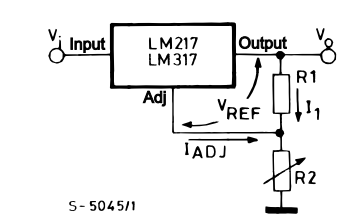
\includegraphics[width=.6\linewidth]{pictures/Lm317 conexionado.PNG}
    \caption{Diagrama de conexionado.}
    \label{fig:kdiagram}
\end{figure}


La ecuación de funcionamiento del regulador que ofrece el fabricante es la siguiente:
\begin{equation}
    V_{OUT} = V_{REF} \cdot ( 1 + \frac{R2}{R1}) + I_{ADJ} \cdot R2
\end{equation}

La ecuación anterior debe ser usada para realizar los cálculos pertinentes sobre el valor de las resistencias R2 y R1. Se pueden realizara además dos observaciones necesarias para la correcta aplicación de la ecuación anterior:
\begin{itemize}
    \item Se tiene que por definición, el fabricante establece el valor $V_{REF}$ en 1.25V
    \item Por motivos de construcción del regulador, la corriente $I_{ADJ}$ tiene un valor máximo de $100 \mu A$ y por lo tanto el término de la ecuación que la involucra puede ser despreciado.
\end{itemize}

Se tiene por lo tanto que la ecuación funcional a utilizar en el cálculo de R1 y R2 es:

\begin{equation}
    V_{OUT} = 1.25 \cdot ( 1 + \frac{R2}{240}) 
\end{equation}

Teniendo en cuenta los voltajes de alimentación requeridos para las dos etapas de alimentación de la PCB, se han realizado los siguientes cálculos para los valores de la resistencia R1 y R2:
\begin{itemize}
    \item Primera etapa, alimentación de servomotores, 5.5V y 0.4A requeridos:
    \begin{equation}
        5.5 = 1.25 \cdot ( 1 + \frac{R2}{R1}) 
    \end{equation}
    Por disponibilidad de materiales, se ha decidido escoger los valores $150 \Omega$ y $500 \Omega$ para los valores de R1 y R2 respectivamente. Tomando en cuenta dichos valores y utilizando la ecuación anterior, se obtiene una reducción de voltaje de 9V a 5.41V, voltaje suficiente para alimentar los servomotores.
\end{itemize}

Aplicando el conexionado recomendado por el fabricante y los cálculos para el valor de las resistencias se obtiene finalmente el diagrama esquemático del circuito de alimentación de los servomotores:

\begin{figure}[H]
    \centering 
    \includegraphics[width=.85\linewidth]{pictures/EsquematicoAlimentaciónServos.PNG}
    \caption{Diagrama esquemático del circuito de alimentación de los servomotores}
    \label{fig:kdiagram}
\end{figure}

El funcionamiento de los reguladores L7805CV y AZ1117H es simple:
\begin{itemize}
    \item El regulador L7805CV recibe un voltaje de entre 7V - 35V y provee un voltaje de salida fijo de 5V. Su conexionado se realiza utilizando dos condensadores auxiliares, tal y como se describe en el datasheet del componente:
    
    \begin{figure}[H]
    \centering 
    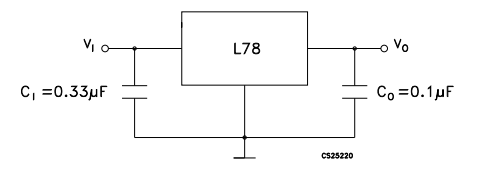
\includegraphics[width=.75\linewidth]{pictures/L7805Datasheet.PNG}
    \caption{Diagrama de conexionado del regulador L7805}
    \label{fig:kdiagram}
    \end{figure}
    
    \item El regulador AZ1117H recibe un voltaje de hasta 15V y provee un voltaje de salida fijo de 3.3V. Su conexionado se realiza de la misma forma que para el regulador anterior, tal y como se describe en el datasheet del componente:
    
    \begin{figure}[H]
    \centering 
    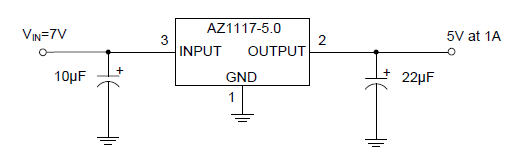
\includegraphics[width=.75\linewidth]{pictures/AZ1117Hdatasheet.PNG}
    \caption{Diagrama de conexionado del regulador AZ1117H}
    \label{fig:kdiagram}
    \end{figure}
    
    En el diagrama anterior se utiliza el modelo que ofrece regulación de voltaje a 5V, sin embargo el modelo usado en el proyecto es el que ofrece regulación de voltaje a 3.3V, siendo su conexionado exactamente igual.
    
\end{itemize}

Teniendo en cuenta la información expuesta anteriormente, se ha decidido conectar en serie ambos reguladores, consiguiendo de esta forma una regulación de 9V a 5V y posteriormente una regulación de 5V a 3.3V. El diagrama esquemático final es el siguiente:

    \begin{figure}[H]
    \centering 
    \includegraphics[width=.95\linewidth]{pictures/EsquematicoAlimentaciónPic.PNG}
    \caption{Diagrama esquemático de la etapa de alimentación del microcontrolador}
    \label{fig:kdiagram}
    \end{figure}

Es importante destacar tres aspectos:
\begin{itemize}
    \item La primera etapa de alimentación incluye clemas para su conexionado con los servomotores.
    \item La segunda etapa de alimentación incluye un puerto de cuatro pines, los cuales se usan para alimentar los micro-interruptores y el microcontrolador.
    \item El conexionado de todos los reguladores se ha realizado en paralelo, dedicando un regulador para cada servomotor, así como para el microcontrolador. El objetivo de esta configuración es garantizar una vía de alimentación independiente para cada componente, reduciendo las interferencias de alimentación entre los reguladores y, diferenciando la etapa de alimentación de los servomotores y microcontrolador.
\end{itemize}

En segundo lugar se procede a describir detalladamente el diagrama esquemático del microcontrolador y sus periféricos. A continuación se muestra el diagrama esquemático final y posteriormente se detallará cada uno de los periféricos:

\begin{figure}[H]
    \centering 
    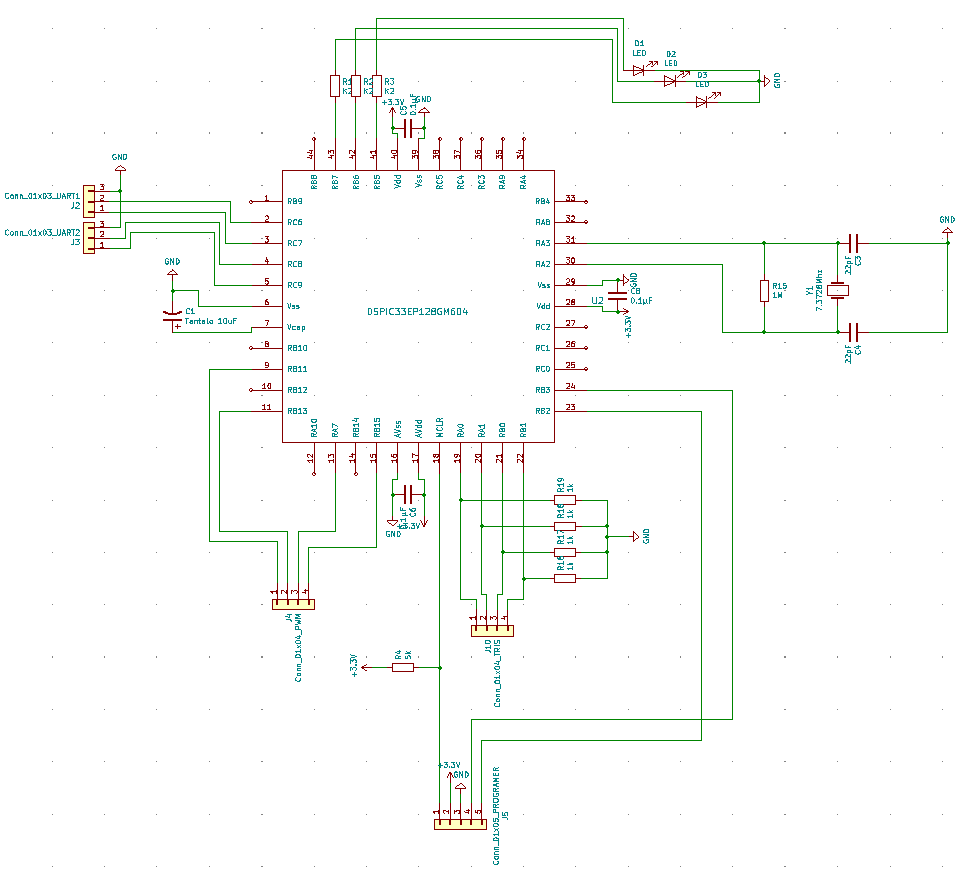
\includegraphics[width=.95\linewidth]{pictures/EsquematicoMicrocontrolador.PNG}
    \caption{Diagrama esquemático del microcontrolador y sus periféricos}
    \label{fig:kdiagram}
\end{figure}

Primeramente es importante describir los condensadores auxiliares necesarios para el correcto funcionamiento del microcontrolador, los cuales se encuentran conectados en los pines de alimentación del mismo. Su conexionado es sugerido por el fabricante en el datasheet según el siguiente esquema, se trata de la configuración mínima recomendada:

\begin{figure}[H]
    \centering 
    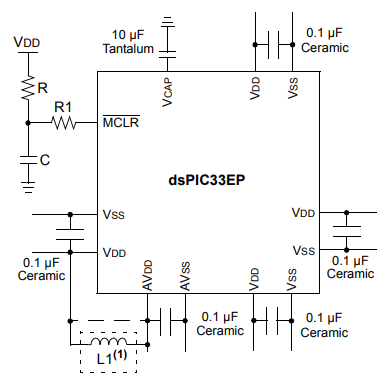
\includegraphics[width=.7\linewidth]{pictures/Minimun.PNG}
    \caption{Conexionado mínimo del microcontrolador}
    \label{fig:kdiagram}
\end{figure}

Todos los condensadores han sido conectados a los pines descritos por el fabricante y escogidos teniendo en cuenta las características técnicas de los mismos, también descritas en el datasheet.

A continuación se describe el conexionado del resto de puertos y periféricos:

\begin{itemize}
    \item Cristal de cuarzo: se trata del periférico que genera la señal de reloj principal del sistema, en este caso, su frecuencia es de 7.3728 Mhz y entra dentro del rango de válido mencionado en el datasheet.
    
    \begin{figure}[H]
    \centering 
    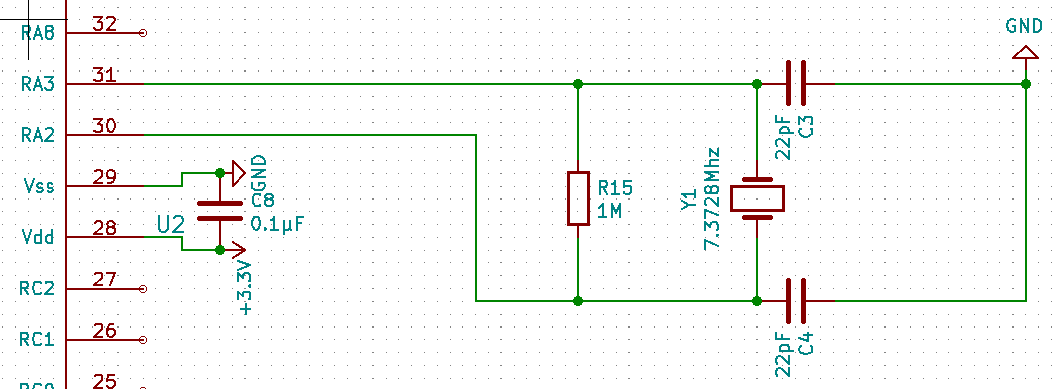
\includegraphics[width=.7\linewidth]{pictures/Cristal.PNG}
    \caption{Diagrama esquemático del conexionado del generador de señales}
    \label{fig:kdiagram}
    \end{figure}
    
    Su conexionado se realiza con los pines 32 y 31 del microcontrolador, siguiendo la estructura de la imagen anterior, empleando también una resistencia de $1 M \Omega$ y dos condensadores de 22 pF.
    
    \item Puerto de programación mediante sonda: se trata del puerto que permite conectar la sonda que introduce el código a ejecutar en el microcontrolador.
    
    El conector que recibe la sonda debe tener una estructura específica y se describe en el datasheet de la misma:
    
    \begin{figure}[H]
    \centering 
    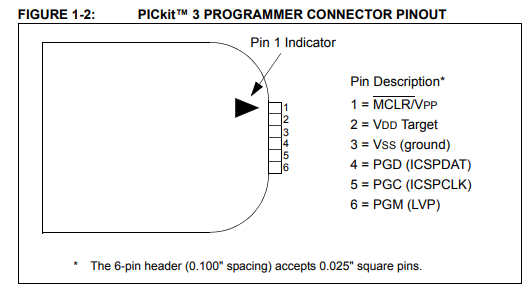
\includegraphics[width=.5\linewidth]{pictures/Sonda.PNG}
    \caption{Pinout del conector de la sonda de programación}
    \label{fig:kdiagram}
    \end{figure}
    
     Cabe destacar que el pin 18 o MCLR debe tener un conexionado específico en el que se emplea una resistencia pull-up; esta estructura de conexión se muestra en el datasheet del microcontrolador:
     
    \begin{figure}[H]
    \centering 
    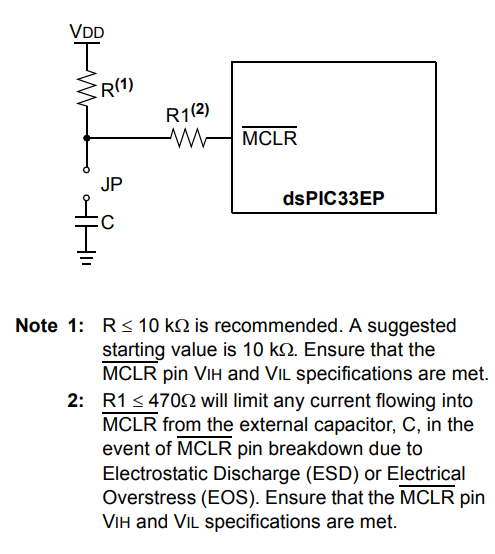
\includegraphics[width=.6\linewidth]{pictures/MCLR.PNG}
    \caption{Conexión del pin MCLR}
    \label{fig:kdiagram}
    \end{figure}
    
    En este proyecto se ha decidido no incluir el jumper sugerido para conexión del pin MCLR y por lo tanto R1 no se incluye en el diagrama esquemático.
    
    Teniendo en cuenta lo anteriormente mencionado, el conexionado final del puerto de programación mediante sonda es el siguiente:
    
    \begin{figure}[H]
    \centering 
    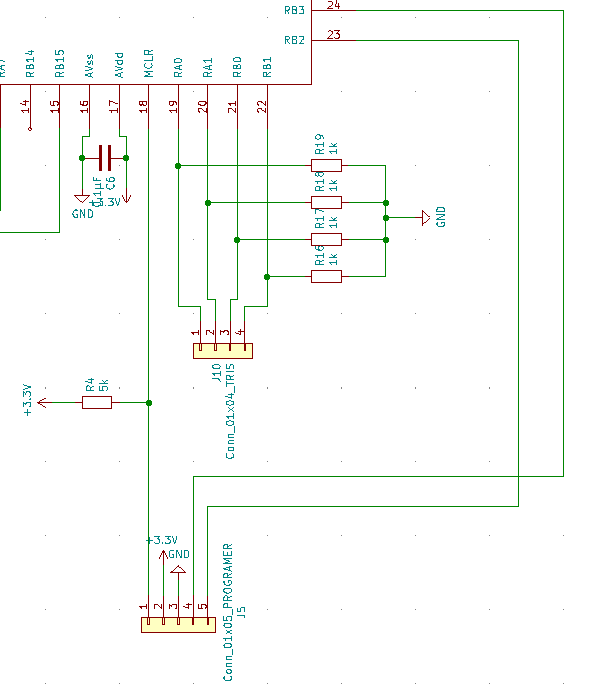
\includegraphics[width=.5\linewidth]{pictures/sonda.PNG}
    \caption{Diagrama esquemático del puerto de programación}
    \label{fig:kdiagram}
    \end{figure}
    
    \item Puerto TRIS: se trata del puerto al que se conectan los micro-interruptores que se utilizan en los finales de carrera de la estructura del brazo robótico.
    
    Para detectar si el brazo robótico se encuentra en uno de sus finales de carrera o zonas límite de movimiento, se utilizan unos micro-interruptores que al ser presionados por el manipulador, realizan cortocircuito. Mediante este cortocircuito y dado que estos micro-interruptores se encuentran conectados a los pines 19, 20, 21 y 22 del microntrolador, se puede realizar la lectura de dichos pines y detectar el estado de micro-interruptor. De esta manera se consigue saber cuando el manipulador ha alcanzado o no un final de carrera.
    
    A continuación se muestra un esquema de lo mencionado anteriormente:
    
    \begin{figure}[H]
    \centering 
    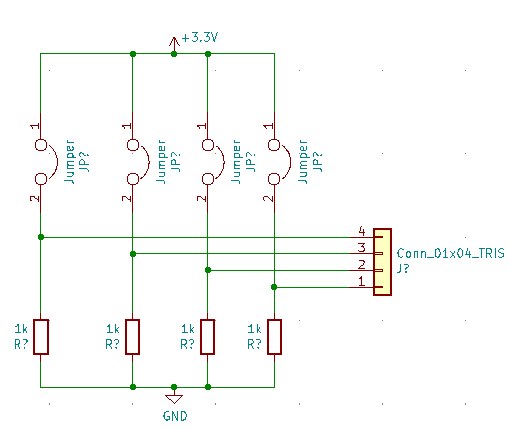
\includegraphics[width=.64
    \linewidth]{pictures/MicroSwitchesSchematic.PNG}
    \caption{Circuito lógico para los finales de carrera}
    \label{fig:kdiagram}
    \end{figure}
    
    Mediante el conexionado anterior, si el micro-interruptor está abierto, se recibe un nivel bajo por el pin del microcontrolador; mientras que si el micro-interruptor está cerrado se recibe un nivel alto por el pin del microcontrolador. 
    
    Cabe destacar que tanto la resistencia pull-down como la conexión a tierra se incluyen en la PCB, sin embargo los micro-interruptores y su conexión a VDD se encuentran localizados en la estructura del brazo robótico. 
    
    El diagrama esquemático que implementa esta funcionalidad es el siguiente:
    
    \begin{figure}[H]
    \centering 
    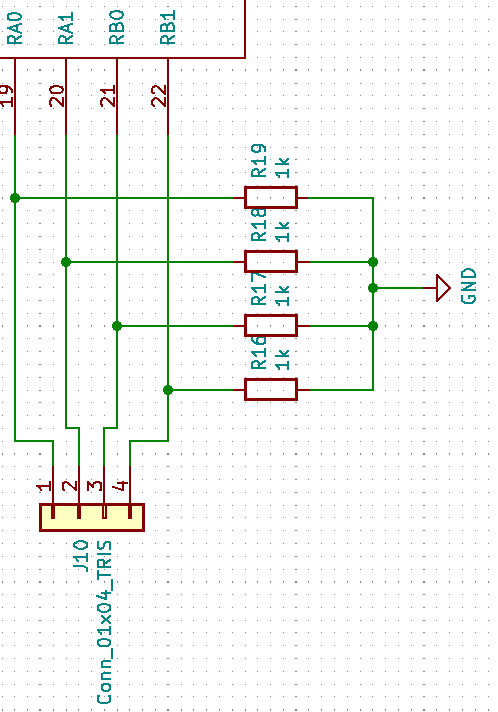
\includegraphics[width=.4\linewidth]{pictures/TRIS.PNG}
    \caption{Diagrama esquemático del puerto TRIS}
    \label{fig:kdiagram}
    \end{figure}
    
    \item Puerto PWM: se trata del puerto que permite utilizar el generador de señales PWM del microcontrolador. 
    
    Dado que en este proyecto se realiza control de servomotores, es completamente necesario el uso de señales PWM para controlar la posición angular de los mismos y por lo tanto se considera a este periférico como uno de los mas relevantes.
    
    Los generadores de señal PWM de este microcontrolador poseen las siguientes características técnicas relevantes:
    \begin{itemize}
        \item El microcontrolador ofrece 6 generadores de señal PWM de alta precisión y velocidad.
        \item Cada uno de los generadores posee un registro de 16 bits para la selección de la duración del ciclo de trabajo; este registro esta divido en parte alta y parte baja.
        \item Es posible utilizar de forma independiente la parte alta y parte baja de cada uno de los generadores, consiguiendo de esta forma dos subgeneradores que producen señales PWM independientes, sin embargo, su precisión se reduce a 8 bits.
    \end{itemize}
    
    El esquema mostrado por el fabricante para los generadores PWM es el siguiente:
    
    \begin{figure}[H]
    \centering 
    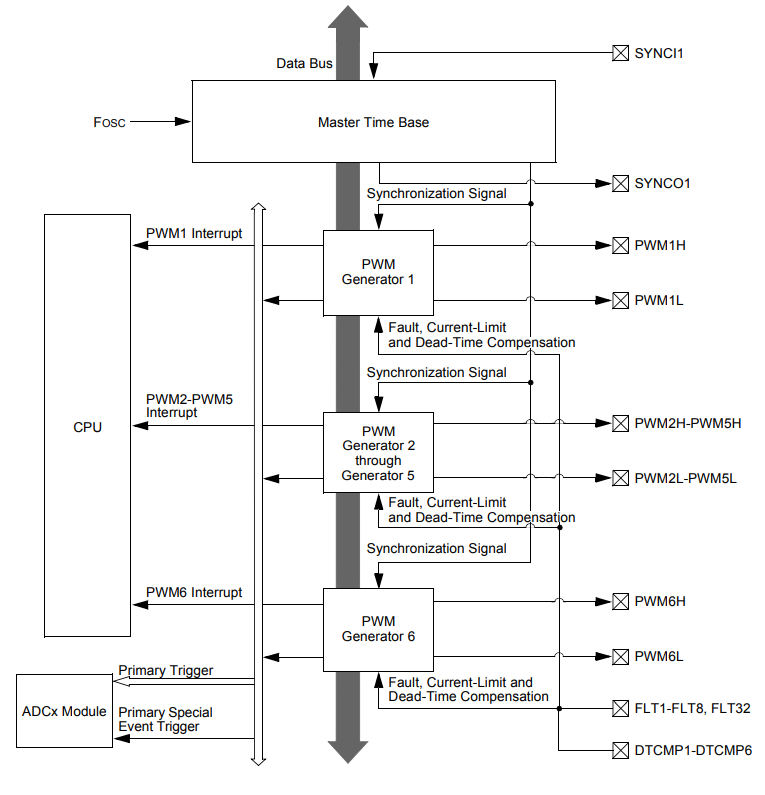
\includegraphics[width=.6\linewidth]{pictures/PWMdatasheet.PNG}
    \caption{Esquema del generador PWM}
    \label{fig:kdiagram}
    \end{figure}
    
    Dado que para este proyecto únicamente se necesitan cuatro generadores PWM, se ha decidido utilizar cuatro módulos con precisión de 16 bits. En el caso de utilizar la precisión completa de cada generador, la señal de salida se proporciona por el pin correspondiente a la parte baja del registro. Mediante la información obtenida del pinout del microcontrolador, se tiene que los generadores de PWM 1, 4, 2 y 3 tienen asignados los pines 15, 13, 11 y 9 respectivamente.
    
    El conexionado final del puerto PWM en el diagrama esquemático es el siguiente:
    
    \begin{figure}[H]
    \centering 
    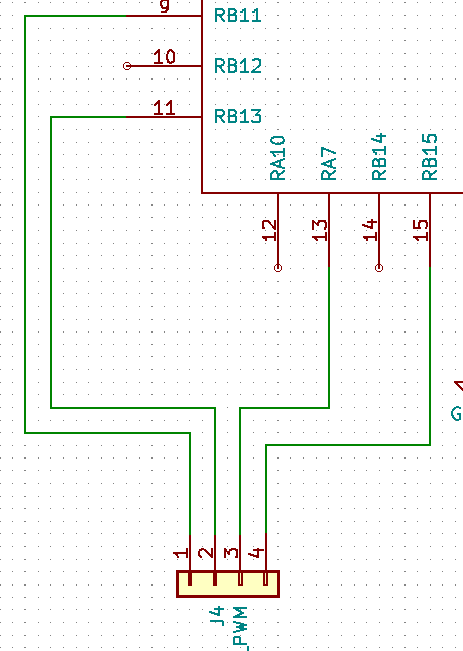
\includegraphics[width=.45\linewidth]{pictures/PWM.PNG}
    \caption{Diagrama esquemático del puerto PWM}
    \label{fig:kdiagram}
    \end{figure}

    \item Puertos UART: se trata de los puertos que permiten la conexión del periférico UART del microcontrolador y mediante los cuales se establece el canal de comunicación con S1.
    
    Mediante el periférico UART se pueden establecer un canal de comunicación hardware asíncrono en el cual existen diversas configuraciones en cuanto a formato de transmisión de bits y velocidades de comunicación. Suele ser un método de comunicación muy usado en microcontroladores y dispositivos hardware en general. El protocolo UART utiliza un puerto con tres conexiones: emisor (TX), receptor(RX) y GND.
    
    El esquema simplificado de este periférico en el datasheet es el siguiente:
    
    \begin{figure}[H]
    \centering 
    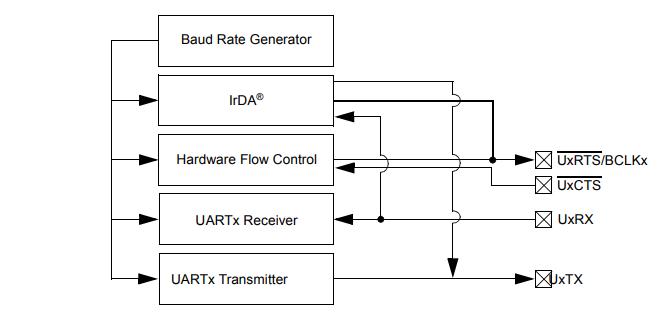
\includegraphics[width=.6\linewidth]{pictures/UARTdatasheet.PNG}
    \caption{Esquema del periférico UART}
    \label{fig:kdiagram}
    \end{figure}
    
    Se ha tomado la decisión de incluir dos puertos UART independientes en la PCB que se ha desarrollado, con el objetivo principalmente de dedicar uno de los canales a envío y recepción de instrucciones; mientras que el otro se usa para realizar labores de depuración y pruebas.
    
    El conexionado de los puertos UART  se realiza mediante pines reconfigurables del microcontrolador, en este caso se han utilizado los pines 2 y 3 para el primer canal; además de los pines 3 y 4 para el segundo canal. El diagrama esquemático final es el siguiente:
    
    \begin{figure}[H]
    \centering 
    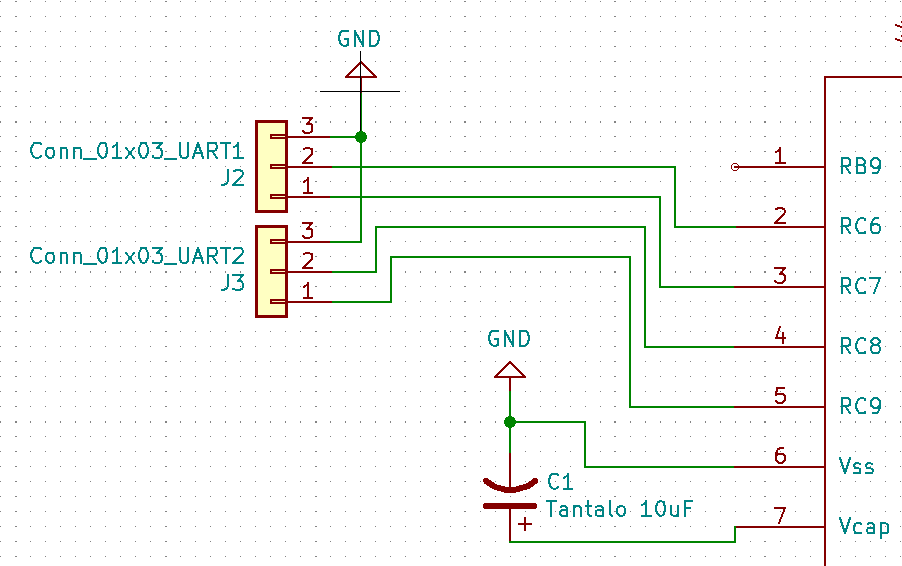
\includegraphics[width=.6\linewidth]{pictures/UART.PNG}
    \caption{Diagrama esquemático de los puertos UART}
    \label{fig:kdiagram}
    \end{figure}
    
    
    \item LEDs de estado: se trata de tres diodos LED que se utilizan para indicar el estado del brazo robótico y demás aspectos del sistema. 
    
    Su conexionado se realizado utilizando los pines reconfigurables 41,42 y 43, los cuales pueden ser usados para habilitar una salida digital. Se considera que un nivel alto enciende el LED mientras que un nivel bajo lo mantiene apagado.
    
    A continuación se muestra el diagrama esquemático del circuito:
    
    \begin{figure}[H]
    \centering 
    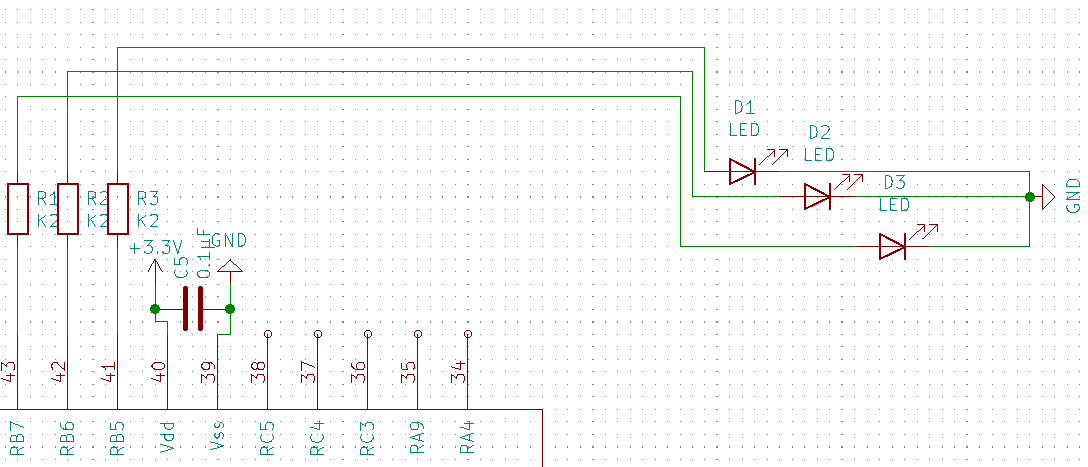
\includegraphics[width=.75\linewidth]{pictures/LEDS.PNG}
    \caption{Diagrama esquemático de los LEDs}
    \label{fig:kdiagram}
    \end{figure}

    Teniendo en cuenta que la corriente máxima suministrada  por el microcontrolador es de 18mA para salida digital y el que voltaje elegido ha sido 3.3V, el pin suministraría como mucho una potencia de 0.0594W. Se ha decidido que una potencia adecuada a suministrar sería un 80\% de la máxima, es decir 0.0475W. Para cumplir esta restricción, se ha calculado el valor ideal de la resistencia del esquema anterior y su valor recomendado es de entre $180 \Omega$ y $200 \Omega$.
    
\end{itemize}

En conclusión, una vista completa sobre el diagrama esquemático del proyecto es la siguiente:

    \begin{figure}[H]
    \centering 
    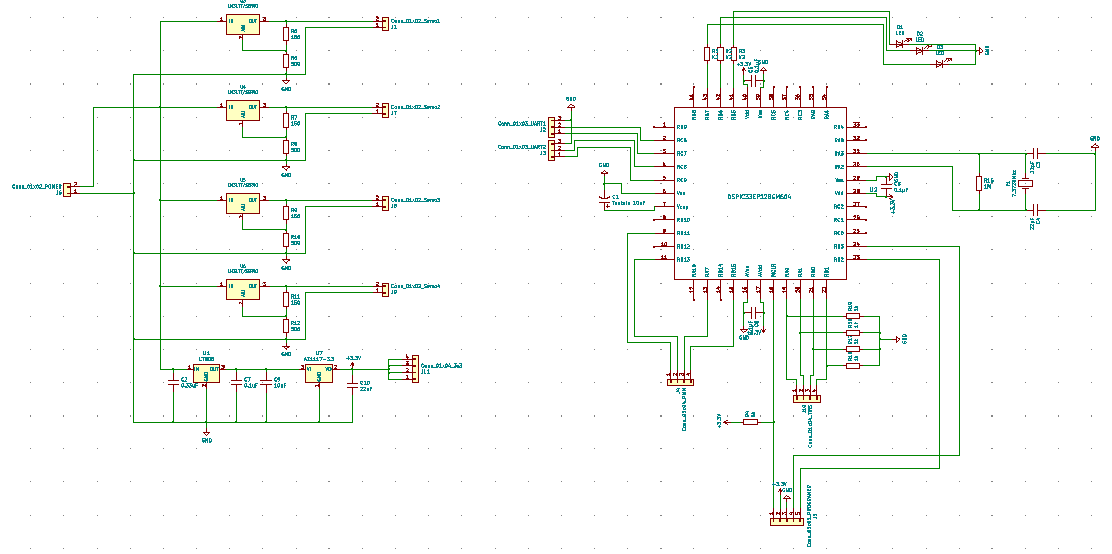
\includegraphics[width=1.05\linewidth]{pictures/EsquematicoCompleto.PNG}
    \caption{Diagrama esquemático de los LEDs}
    \label{fig:kdiagram}
    \end{figure}

\subsection{Diseño y Diagrama físico}

Tal y como se ha descrito en el apartado anterior, el diseño lógico de la PCB se implementa mediante el diagrama esquemático, y su objetivo es el de describir las huellas y conexiones lógicas de los componentes; sin embargo, este diseño es de alto nivel y no es implementable directamente en términos físicos. 

El siguiente paso tras completar el diagrama esquemático es transformar este diseño lógico en un diseño físico mas cercano a la implementación real. 

El diseño físico de una PCB debe ser obtenido directamente de la información establecida en el diseño lógico y por lo tanto, se tiene que transformar el diseño esquemático en un diseño físico, en el cual se deben contemplar los aspectos físicos de los componentes y sus conexiones, además de sus aspectos lógicos.

El objetivo principal del diseño y diagrama físico es el de plasmar la realidad física de los componentes y sus conexiones a partir de un diagrama esquemático, en el cual no se contemplan los aspectos físicos para simplificar el diseño inicial. En general, el diseño y diagrama físico es más complejo y difícil de comprender, por ello, normalmente, la primera etapa del diseño comienza con el diseño lógico y diagrama esquemático.



\subsection{Conexionado y enrutado mediante pistas}

\subsection{Verificaciones del diseño final}

\subsection{Decisiones críticas durante el desarrollo}

\subsection{Construcción}

